\pdfoutput=1
\documentclass[a4paper,pdflatex,ja=standard]{bxjsarticle}

% ---Setting about the geometry of the document----
% \usepackage{a4wide}
% \pagestyle{empty}

% ---Physics and Math Packages---
\usepackage{amssymb,amsfonts,amsthm,mathtools}
\usepackage{physics,braket,bm}

% ---underline---
\usepackage{ulem}

% --- sorround the texts or equations
% \usepackage{fancybox,ascmac}

% ---settings of theorem environment---
% \usepackage{amsthm}
% \theoremstyle{definition}

% ---settings of proof environment---
% \renewcommand{\proofname}{\textbf{証明}}
% \renewcommand{\qedsymbol}{$\blacksquare$}

% ---Ignore the Warnings---
\usepackage{silence}
\WarningFilter{latexfont}{Some font shapes,Font shape}

% ---Insert the figure (If insert the `draft' at the option, the process becomes faster)---
\usepackage{graphicx}
% \usepackage{subcaption}

% ----Add a link to a text---
\usepackage{url}
\usepackage{xcolor,hyperref}
\hypersetup{colorlinks=true,citecolor=orange,linkcolor=blue,urlcolor=magenta}
\usepackage{bxcjkjatype}

% ---Tikz---
\usepackage{tikz,pgf,pgfplots,circuitikz}
\pgfplotsset{compat=1.15}
\usetikzlibrary{intersections,arrows.meta,angles,calc,3d,decorations.pathmorphing}

% ---Add the section number to the equation, figure, and table number---
\makeatletter
   \renewcommand{\theequation}{\thesection.\arabic{equation}}
   \@addtoreset{equation}{section}
   
   \renewcommand{\thefigure}{\thesection.\arabic{figure}}
   \@addtoreset{figure}{section}
   
   \renewcommand{\thetable}{\thesection.\arabic{table}}
   \@addtoreset{table}{section}
\makeatother

% ---enumerate---
\renewcommand{\labelenumi}{\arabic{enumi}.}
\renewcommand{\labelenumii}{(\roman{enumii})}

% ---Index---
% \usepackage{makeidx}
% \makeindex 

% ---Fonts---
\renewcommand{\familydefault}{\sfdefault}

% ---Title---
\title{東京大学\ 令和4年\ 物理学専攻\ 院試\ 解答例}
\author{ミヤネ}
\date{最終更新:\today}

\newcommand{\prb}[2]{
  \phantomsection
  \addcontentsline{toc}{section}{問題 #1: #2}
  \section*{第#1問}
  \setcounter{section}{#1}
  \setcounter{equation}{0}
}

\begin{document}

\maketitle

\tableofcontents
\clearpage

\setcounter{section}{1}

\prb{1}{量子力学}
\begin{enumerate}
  \item 
  $\ev*{\hat{x}},\ev*{\hat{p}}$をそれぞれ計算すると
  \begin{align}
    \ev*{\hat{x}}
    &=
    \int_{-\infty}^{\infty}\overline{\psi}(x)\hat{x}\psi(x) \dd x
    \nonumber
    \\
    &=
    \frac{1}{\sqrt{\pi a^2}}\int_{-\infty}^{\infty} xe^{-x^2/a^2}\dd x
    \nonumber
    \\
    &=
    0
    \\
    \ev*{\hat{p}}
    &=
    \int_{-\infty}^{\infty}\overline{\psi}(x)\hat{p}\psi(x) \dd x
    \nonumber
    \\
    &=
    \frac{i\hbar}{a^2\sqrt{\pi a^2}}\int_{-\infty}^{\infty}xe^{-x^2/a^2}\dd x
    \nonumber
    \\
    &=
    0
  \end{align}
  となる.よって,
  \begin{align}
    (\Delta x)^2
    &=
    \ev*{\hat{x}^2}
    \nonumber
    \\
    &=
    \frac{1}{\sqrt{\pi a^2}}\int_{-\infty}^{\infty} x^{2}e^{-x^2/a^2}\dd x
    \nonumber
    \\
    &=
    \frac{a^2}{2}
    \\
    (\Delta p)^2
    &=
    \ev*{\hat{p}^2}
    \nonumber
    \\
    &=
    \frac{1}{\sqrt{\pi a^2}}\int_{-\infty}^{\infty} \hat{p}^{2}e^{-x^2/a^2}\dd x
    \nonumber
    \\
    &=
    \frac{\hbar^2}{2a^2}
  \end{align}
  である.したがって,
  \begin{equation}
    \Delta x = \frac{a}{\sqrt{2}}
    \ ,\ \ 
    \Delta p = \frac{\hbar}{\sqrt{2}a}
  \end{equation}
  であり,これらの積は
  \begin{equation}
    \Delta x\Delta p
    =
    \frac{\hbar}{2}
  \end{equation}
  となり,これはここで用いた波動関数が不確定性が最小であることを意味している.

  \item 
  $\hat{\mathcal{O}}^{\dagger}\hat{\mathcal{O}}$の期待値を計算すると
  \begin{align}
    \ev*{\hat{\mathcal{O}}^{\dagger}\hat{\mathcal{O}}}
    &=
    \int_{-\infty}^{\infty}\overline{\psi}(x)\hat{\mathcal{O}}^{\dagger}\hat{\mathcal{O}}\psi(x) \dd x
    \nonumber
    \\
    &=
    \int_{-\infty}^{\infty}\|\hat{\mathcal{O}}\psi(x)\|^2 \dd x \geq 0
    \label{O_times_wavefunction}
  \end{align}
  となる.

  \item 
  $\hat{\mathcal{O}}=t\Delta \hat{x}-i\Delta \hat{p}$とすると,
  \begin{align}
    \ev*{\hat{\mathcal{O}}^{\dagger}\hat{\mathcal{O}}}
    &=
    \ev*{\left( t\Delta\hat{x}+i\Delta\hat{p} \right)\left( t\Delta\hat{x}-i\Delta\hat{p} \right)}
    \nonumber
    \\
    &=
    t^2\ev*{(\Delta\hat{x})^2}
    -
    \ev*{it\left[ \Delta\hat{x}, \Delta\hat{p} \right]}
    +
    \ev*{(\Delta\hat{p})^2}
    \nonumber
    \\
    &=
    \Delta x^2 t^2
    +
    \hbar t
    +
    \Delta p^2
  \end{align}
  なので,前問より,不等式
  \begin{equation}
    \Delta x^2 t^2
    +
    \hbar t
    +
    \Delta p^2
    \geq 
    0
  \end{equation}
  が任意の$t$について成立する.したがって,そのためには判別式$D$について
  \begin{equation}
    D
    \coloneqq
    \hbar^2 - 4 \Delta x^2 \Delta p^2
    \leq
    0
  \end{equation}
  となっていればよいので
  \begin{equation}
    \Delta x\Delta p\geq \frac{\hbar}{2}
  \end{equation}
  が示された.

  \item 
  \eqref{O_times_wavefunction}は
  \begin{equation}
    \int_{-\infty}^{\infty}\|\hat{\mathcal{O}}\psi(x)\|^2 \dd x \geq 0
  \end{equation}
  であった.固有値が$0$であるためには,この不等式の等号が成立していればよい.よって,この不等式が常に成立していることに注意すれば,方程式
  \begin{equation}
    \Delta x^2 t^2
    +
    \hbar t
    +
    \Delta p^2
    =
    0
  \end{equation}
  が重解をもつことがわかり,それは
  \begin{equation}
    t
    =
    -\frac{\hbar}{2\Delta x^2}
    \label{t_dup}
  \end{equation}
  である.

  \item 
  \eqref{t_dup}のとき,波動関数$\psi(x)$の固有値が$0$より
  \begin{equation}
    -\frac{\hbar}{2\Delta x^2}
    (x-\ev*{\hat{x}})\psi(x)
    -i
    \left(  
      -i\hbar\dv{}{x}-\ev*{\hat{p}}
    \right)
    \psi(x)
    =
    0
  \end{equation}  
  なので,これを整理すれば
  \begin{equation}
    \dv{}{x}\psi(x)
    =
    -\frac{1}{2\Delta x^2}
    \left( 
      x-\ev*{\hat{x}}-\frac{2i\Delta x^2}{\hbar}\ev*{\hat{p}}
    \right)\psi(x)
  \end{equation}
  となる.これを解けば
  \begin{equation}
    \psi(x)
    =
    A \exp\left[ -\frac{1}{4\Delta x^2}
    \left( 
      x-\ev*{\hat{x}}-\frac{2i\Delta x^2}{\hbar}\ev*{\hat{p}}
    \right)^2 \right]
  \end{equation}
  となる.ここで,$A$は定数である.これを規格化すると
  \begin{equation}
    \int_{-\infty}^{\infty}
    \overline{\psi}(x)\psi(x)\dd x
    =
    |A|^2
    \int_{-\infty}^{\infty}\dd x\ 
    \exp\left[ -\frac{1}{2\Delta x^2}x^2 \right]
    =
    |A|^2\sqrt{2\pi\Delta x^2}
    =
    1
  \end{equation}
  となるので
  \begin{equation}
    \psi(x)
    =
    \left( \frac{1}{2\pi\Delta x^2} \right)^{1/4}
    \exp\left[ -\frac{1}{4\Delta x^2}
    \left( 
      x-\ev*{\hat{x}}-\frac{2i\Delta x^2}{\hbar}\ev*{\hat{p}}
    \right)^2 \right]
  \end{equation}
  がもとめる規格化された波動関数である.
\end{enumerate}

\clearpage
\prb{2}{統計力学}
\begin{enumerate}
  \item 
  シュレーディンガー方程式は
  \begin{equation}
    -\frac{\hbar^2}{2m}\left( \pdv[2]{}{x}+\pdv[2]{}{y}+\pdv[2]{}{z} \right)\Psi(x,y,z)
    =
    E\Psi(x,y,z)
  \end{equation}
  である.ここで,
  \begin{equation}
    \Psi(x,y,z)
    \coloneqq
    \psi_{x}(x)\psi_{y}(y)\psi_{z}(z)
  \end{equation}
  と変数分離すると
  \begin{equation}
    \left\{\begin{alignedat}{1}
      -\frac{\hbar^2}{2m}\dv[2]{}{x}\psi_{x}(x)=E_{x}\psi_{x}(x)
      \\
      -\frac{\hbar^2}{2m}\dv[2]{}{y}\psi_{y}(y)=E_{y}\psi_{y}(y)
      \\
      -\frac{\hbar^2}{2m}\dv[2]{}{z}\psi_{z}(z)=E_{z}\psi_{z}(z)
      \\
      E\eqcolon E_{x}+E_{y}+E_{z}
    \end{alignedat}\right.
  \end{equation}
  となる.$x$について解くと,一般解は
  \begin{equation}
    \psi_{x}(x)
    =
    Ae^{ik_{x}x}+Be^{-ik_{x}x}
  \end{equation}
  である.ただし
  \begin{equation}
    k_{x}
    \coloneqq
    \sqrt{\frac{2mE_{x}}{\hbar^2}}
  \end{equation}
  とおいた.ここで,周期境界条件として$\psi_{x}(x)=\psi_{x}(x+L)$を考えると,
  \begin{equation}
    k_x L
    =
    2n_x\pi
  \end{equation}
  であり,エネルギーは
  \begin{equation}
    E_x
    =
    \frac{2\pi^2\hbar^2}{mL^2}n_x^2
  \end{equation}
  となる.このときの規格化条件は
  \begin{equation}
    \int_{0}^{L}
    \psi_x^{*}(x)\psi_x(x)
    \dd x
    =
    L\left( |A|^2+|B|^2 \right)
    =
    1
  \end{equation}
  であり,$B=0$だとすれば\footnote{
    たぶん,$A,\ B$についての任意性はあると思います.
  }
  \begin{equation}
    \psi_x(x)
    =
    \frac{1}{\sqrt{L}}e^{ik_xx}
  \end{equation}
  と規格化される.したがって,固有波動関数は
  \begin{equation}
    \Psi(x,y,z)
    =
    \frac{1}{L^{3/2}}e^{i(k_xx+k_yy+k_zz)}
  \end{equation}
  であり,固有エネルギーは
  \begin{equation}
    E
    =
    \frac{2\pi^2\hbar^2}{mL^2}(n_x^2+n_y^2+n_z^2)
  \end{equation}
  である.

  \item 
  次の不等式
  \begin{equation}
    \frac{2\pi^2\hbar^2}{mL^2}
    \left( n_{x}^2+n_{y}^2+n_{z}^2 \right)
    \leq
    E
  \end{equation}
  つまり
  \begin{equation}
    n_{x}^2+n_{y}^2+n_{z}^2
    \leq
    \frac{mL^2}{2\pi^2\hbar^2}
    E
  \end{equation}
  を満たす$(n_{x},n_{y},n_{x})$の組の個数をもとめればよい.$L$が大きいとき,これは半径$\sqrt{mL^2/2\pi^2\hbar^2}$の球の体積に近似できるので
  \begin{equation}
    \Omega(E)
    =
    \frac{4\pi}{3}
    \left(  
      \frac{mL^2}{2\pi^2\hbar^2}
      E
    \right)^{3/2}
  \end{equation}
  である.よって
  \begin{equation}
    D(E)
    =
    2\pi\sqrt{E}
    \left(  \frac{2\pi^2\hbar^2}{mL^2}  \right)^{3/2}
    =
    2\pi
    \left(  
      \frac{mL^2}{2\pi^2\hbar^2}
    \right)^{3/2}
    E^{1/2}
    \label{state}
  \end{equation}
  である.

  \item 
  $\mu=0$のときは
  \begin{align}
    \int_{0}^{\infty}f(E,0)D(E)\dd E
    &=    
    2\pi\left( \frac{mL^2}{2\pi^2\hbar^2} \right)
    \int_{0}^{\infty}
    \frac{\sqrt{E}}{e^{E/k_BT}-1}
    \dd E
    \nonumber
    \\
    &=
    V
    \left(  
      \frac{mk_BT}{2\pi\hbar^2}
    \right)^{3/2}
    \zeta\left( \frac{3}{2} \right)
    \label{ans2.4}
  \end{align}
  である.

  \item 
  粒子数は
  \begin{equation}
    N
    =
    \left\{\begin{alignedat}{1}
      \int_{0}^{\infty}f(E,\mu)D(E)\dd E
      &
      (T_{c}<T)
      \\
      N_{0}+\int_{0}^{\infty}f(E,0)D(E)\dd E
      &
      (T_{c}\geq T)
    \end{alignedat}\right.
  \end{equation}
  となっている.$T=T_c$のときは,ちょうど$N_{0}=0$となるので
  \begin{equation}
    N
    =
    \int_{0}^{\infty}f(E,0)D(E)\dd E
  \end{equation}
  となっているので,
  \begin{equation}
    N
    =
    V
    \left(  
      \frac{mk_BT_c}{2\pi\hbar^2}
    \right)^{3/2}
    \zeta\left( \frac{3}{2} \right)
    \label{number_critical}
  \end{equation}
  である.これを$T_{c}$について解けば
  \begin{equation}
    T_{c}
    =
    \frac{2\pi\hbar^2}{mk_B}
    \left(  
      \frac{N}{V\zeta(3/2)}
    \right)^{2/3}
  \end{equation}
  である.

  \item 
  $T<T_{c}$のときは,\eqref{ans2.4}により
  \begin{gather}
    N
    =
    N_{0}
    +
    C\times T^{3/2}
    \\
    C\coloneqq
    V
    \left(  
      \frac{mk_B}{2\pi\hbar^2}
    \right)^{3/2}
    \zeta\left( \frac{3}{2} \right)
  \end{gather}
  であることがわかる.ただし,$T$に依存しない係数は$C$でまとめた.$T=T_{c}$では,同様にして
  \begin{equation}
    N=C\times T_{c}^{3/2}
  \end{equation}
  が成立したのでこれらを連立して,$C$を消去すれば
  \begin{equation}
    N=N_{0}+N\left( \frac{T}{T_{c}} \right)^{3/2}
  \end{equation}
  となるので
  \begin{equation}
    N_{0}
    =
    N\left\{ 1-\left( \frac{T}{T_{c}} \right)^{3/2} \right\}
  \end{equation}
  である.

  \item 
  エネルギーは
  \begin{equation}
    E
    =
    \int_{0}^{\infty}\dd \varepsilon\ \varepsilon f(\varepsilon,0)D(\varepsilon)
  \end{equation}
  でもとめることができるので,これを計算すると
  \begin{equation}
    E
    \propto
    T^{5/2}
  \end{equation}
  と書けるので
  \begin{equation}
    C_{V}\propto T^{3/2}
  \end{equation}
  となる.よって
  \begin{equation}
    \gamma=\frac{3}{2}
  \end{equation}
  ともとまった.

  \item 
  一般に縮退度を$g$とすると,ひとつの自由度に対して状態数が決まるので\eqref{state}は
  \begin{equation}
    \frac{D(E)}{g}
    =
    2\pi
    \left(  
      \frac{mL^2}{2\pi^2\hbar^2}
    \right)^{3/2}
    E^{1/2}
  \end{equation}
  と書ける.よって,スピンが$S$の場合は縮退度は$g=2S+1$なので
  \begin{equation}
    D(E)
    =
    2\pi(2S+1)
    \left(  
      \frac{mL^2}{2\pi^2\hbar^2}
    \right)^{3/2}
    E^{1/2}
  \end{equation}
  である.したがって,転移温度での粒子数は\eqref{number_critical}から
  \begin{equation}
    N
    =
    V(2S+1)
    \left(  
      \frac{mk_BT_c^{\prime}}{2\pi\hbar^2}
    \right)^{3/2}
    \zeta\left( \frac{3}{2} \right)
  \end{equation}
  となるので
  \begin{equation}
    T_{c}^{\prime}
    =
    \frac{2\pi\hbar^2}{mk_B}
    \left(  
      \frac{N}{(2S+1)V\zeta(3/2)}
    \right)^{2/3}
  \end{equation}
  である.

  \item 
  スピンが$m_z$の粒子の状態密度を$D_{m_z}$とする.このとき,状態密度は
  \begin{equation}
    D_{m_z}(E)
    =
    D(E+cm_{z}B)
    =
    2\pi V
    \left(  
      \frac{m}{2\pi^2\hbar^2}
    \right)^{3/2}
    \sqrt{E+cm_{z}B}
  \end{equation}
  と書ける.スピンが$m_z$の粒子の転移温度における粒子数が
  \begin{equation}
    N_{m_{z}}
    =
    \int_{0}^{\infty}f(E,0)D_{m_z}(E)\dd E
    \label{num_mz}
  \end{equation}
  とかけるので,全粒子数は
  \begin{equation}
    N
    =
    \sum_{m_z=-S}^{S}\int_{0}^{\infty}f(E,0)D_{m_z}(E)\dd E
    \label{num_tot}
  \end{equation}
  である.\eqref{num_mz}を計算してみると
  \begin{align}
    N_{m_{z}}
    &=
    \int_{0}^{\infty}f(E,0)D(E+cm_{z}B)\dd E
    \nonumber
    \\
    &=
    2\pi V
    \left(  
      \frac{m}{2\pi^2\hbar^2}
    \right)^{3/2}
    \int_{0}^{\infty}
    \frac{\sqrt{E+cm_{z}B}}{e^{E/k_{B}T_{c}^{\prime}}-1}    
    \dd E
  \end{align}
  となるので,転移温度$T_{c}^{\prime}$を決定する方程式は\eqref{num_tot}より
  \begin{equation}
    N
    =
    2\pi V
    \left(  
      \frac{m}{2\pi^2\hbar^2}
    \right)^{3/2}
    \sum_{m_z=-S}^{S}
    \int_{0}^{\infty}
    \frac{\sqrt{E+cm_{z}B}}{e^{E/k_{B}T_{c}^{\prime}}-1}    
    \dd E
    \label{num_tot2}
  \end{equation}
  となる.
  
  \item 
  \eqref{num_tot2}の積分は,$cB\gg k_{B}T_{c}^{\prime}$の近似をもちいれば
  \begin{equation}
    e^{E/k_{B}T_{c}^{\prime}}-1
    \sim
    e^{E/k_{B}T_{c}^{\prime}}
  \end{equation}
  となるので
  \begin{align}
    \sqrt{k_{B}T_{c}^{\prime}}\cdot\int_{0}^{\infty}\frac{\sqrt{E/k_{B}T_{c}^{\prime}+cm_{z}B/k_{B}T_{c}^{\prime}}}{e^{E/k_{B}T_{c}^{\prime}}-1}\dd E
    &\sim
    \sqrt{k_{B}T_{c}^{\prime}}\cdot\int_{0}^{\infty}\sqrt{E/k_{B}T_{c}^{\prime}+cm_{z}B/k_{B}T_{c}^{\prime}}e^{-E/k_{B}T_{c}^{\prime}}\dd E
    \nonumber
    \\
    &=
    (k_{B}T_{c}^{\prime})^{3/2}e^{cm_{z}B/k_B T}\int_{0}^{\infty}\sqrt{x}e^{-x}\dd x
    \nonumber
    \\
    &=
    \frac{\sqrt{\pi}}{2}(k_{B}T_{c}^{\prime})^{3/2}e^{cm_{z}B/k_B T}
  \end{align}
  である.よって,\eqref{num_tot2}は
  \begin{align}
    N
    &=
    2\pi V
    \left(  
      \frac{m}{2\pi^2\hbar^2}
    \right)^{3/2}
    \cdot
    \frac{\sqrt{\pi}}{2}(k_{B}T_{c}^{\prime})^{3/2}\sum_{m_z=-S}^{S}e^{cm_{z}B/k_B T}
    \nonumber
    \\
    &=
    V
    \left(  
      \frac{mk_BT_c'}{2\pi^2\hbar^2}
    \right)^{3/2}
    \cdot
    \frac{1-e^{c(2S+1)B/k_{B}T_{c}^{\prime}}}{1-e^{cB/k_{B}T_{c}^{\prime}}}e^{-cSB/k_{B}T_{c}^{\prime}}
    \nonumber
    \\
    &\sim
    V
    \left(  
      \frac{mk_BT_c'}{2\pi^2\hbar^2}
    \right)^{3/2}
    \cdot
    e^{-cSB/k_{B}T_{c}^{\prime}}
  \end{align}
  である\footnote{
    最後の行では,$cB/k_BT_c'\gg 1$より
    $$
      (\text{分母})
      \sim
      -e^{cB/k_BT_c'}
      ,\ 
      (\text{分子})
      \sim
      -e^{c(2S+1)B/k_BT_c'}  
    $$
    としました.
  }.両辺の自然対数$\log$をとって,整理すると
  \begin{equation}
    \frac{cSB}{k_{B}}
    \cdot
    \frac{1}{T_{c}^{\prime}}
    =
    \frac{3}{2}
    \log
    \left[  
      \frac{mk_BT_c'}{2\pi^2\hbar^2}\left( \frac{V}{N} \right)^{2/3}
    \right]
  \end{equation}
  となる.ここで,$T_{c}^{\prime}$について左辺は双曲線であり,右辺は対数関数となっている.この2つのグラフの交点が転移温度$T_{c}^{\prime}$である.
  \begin{figure}[ht]
    \centering    
    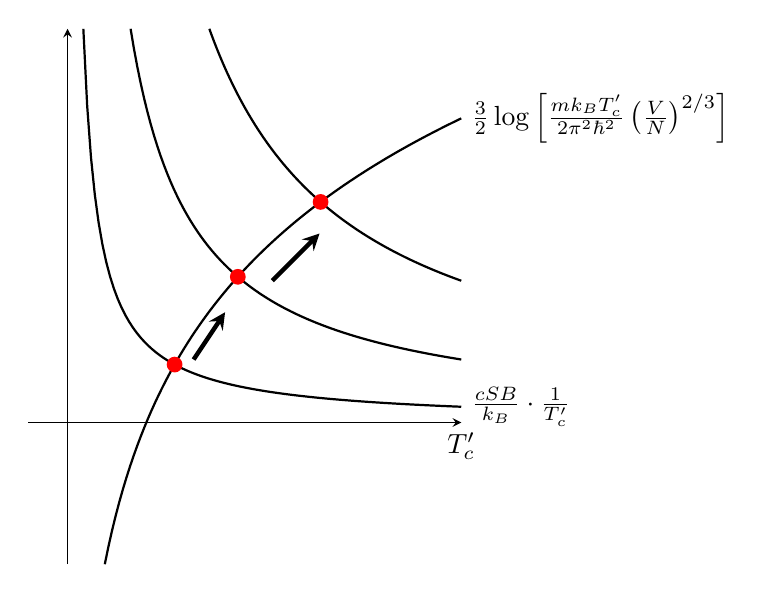
\begin{tikzpicture}
      \draw[->,>=stealth](-0.5,0)--(5.0,0)node[below]{$T_{c}^{\prime}$};
      \draw[->,>=stealth](0,-1.8)--(0,5.0);
      \draw[thick,samples=100,domain=exp(-1.8/2.4):5,name path=A]plot(\x,{2.4*ln(\x)})node[right]{$
        \frac{3}{2}
        \log
        \left[  
          \frac{mk_BT_c'}{2\pi^2\hbar^2}\left( \frac{V}{N} \right)^{2/3}
        \right]
      $};
      \draw[thick,samples=100,domain=1/5:5,name path=B]plot(\x,{1/(\x)})node[right]{$\frac{cSB}{k_{B}}\cdot\frac{1}{T_{c}^{\prime}}$};
      \draw[thick,samples=100,domain=4/5:5,name path=C]plot(\x,{4/(\x)});
      \draw[thick,samples=100,domain=9/5:5,name path=D]plot(\x,{9/(\x)});
      \path[name intersections={of= A and B, by=E}];
      \path[name intersections={of= A and C, by=F}];
      \path[name intersections={of= A and D, by=G}];
      \fill[red](E)circle(0.1);
      \fill[red](F)circle(0.1);          
      \fill[red](G)circle(0.1);
      \draw[->,>=stealth,ultra thick](1.6,0.8)--(2.0,1.4);
      \draw[->,>=stealth,ultra thick](2.6,1.8)--(3.2,2.4);
    \end{tikzpicture}
    \caption{転移温度$T_{c}^{\prime}$を求める方法($B$が大きくなると転移温度も赤点のように遷移する)}    
    \label{fig}
  \end{figure}
  図\ref{fig}を見ればわかるように,磁場$B$が増加すれば,転移温度も緩やかに増加することが読みとれる.よって,転移温度$T_{c}^{\prime}$と磁場$B$の関係は,図\ref{fig_ans}のようになる\footnote{
    $B=0$のときは,
    $$
      T_c'
      =
      \frac{2\pi^2\hbar^2}{mk_B}
      \left(  
        \frac{N}{V}
      \right)^{2/3}
    $$
    です.
  }.
  \begin{figure}[ht]
    \centering    
    \begin{tikzpicture}
      \draw[->,>=stealth](-0.4,0)--(5.0,0)node[below]{$B$};
      \draw[->,>=stealth](0,-0.2)--(0,3.0)node[above right]{$T_{c}^{\prime}$};
      \draw[thick,samples=100,domain=0:5,name path=A]plot(\x,{ln(\x+2)});
      \draw(0,1)node[left]{$
        \frac{2\pi^2\hbar^2}{mk_B}
        \left(  
          \frac{N}{V}
        \right)^{2/3}
      $};
    \end{tikzpicture}
    \caption{転移温度$T_{c}^{\prime}$と磁場$B$の関係}    
    \label{fig_ans}
  \end{figure}

\end{enumerate}

\clearpage
\prb{3}{電磁気学}
\begin{enumerate}
  \item 
  $\bm{\nabla}\times\bm{E}$は$x$成分しか成分をもたないことので,$\bm{B}_{0}$も$x$成分しか成分をもたない.$x$成分については
  \begin{equation}
    kE_{0}\sin(kz-\omega t)=-\omega B_{0}\sin(kz-\omega t)
  \end{equation}
  が成立しているので,これを解けば$B_{0}=-E_{0}/v$である.よって
  \begin{equation}
    \bm{B}_{0}
    =
    (-E_{0}/v,0,0)
  \end{equation}
  である.

  \item
  電磁波の速さ$v$は
  \begin{equation}
    v=\frac{1}{\sqrt{\varepsilon\mu}}
  \end{equation}
  であることが,マクスウェル方程式からわかる.透磁率が一定の場合,速さが2倍になるためには,誘電率は1/4倍にならなくてはならない.

  \item 
  電場と磁場をすべて書くと
  \begin{align}
    &
    \bm{E}_{1}
    =
    (0,E_{0}\cos(kz-\omega t),0)
    \\
    &
    \bm{E}_{2}
    =
    (0,T\cos(kz/2-\omega t),0)
    \\
    &
    \bm{E}_{1}
    =
    (0,R\cos(-kz-\omega t),0)
    \\
    &
    \bm{B}_{1}
    =
    (-E_{0}/v\cos(kz-\omega t),0,0)
    \\
    &
    \bm{B}_{2}
    =
    (-T/2v\cos(kz/2-\omega t),0,0)
    \\
    &
    \bm{B}_{3}
    =
    (R/v\cos(-kz-\omega t),0,0)
  \end{align}
  である.よって,$z=0$での境界条件は
  \begin{equation}
    \left\{\begin{alignedat}{1}
      \text{電場:}&\ 
      E_{0} + R = T
      \\
      \text{磁場:}&\  
      -\frac{E_{0}}{v}
      +\frac{R}{v}
      =
      -\frac{T}{2v}
    \end{alignedat}\right.
  \end{equation}
  となる.これを解けば
  \begin{equation}
    \frac{T}{E_{0}}
    =
    \frac{4}{3}
    \ ,\ \ 
    \frac{R}{E_{0}}
    =
    -\frac{1}{3}
  \end{equation}
  となる.

  \item 
  電場$\bm{E}_{1},\bm{E}_{2}$は
  \begin{align}
    &
    \bm{E}_{1}
    =
    (0,E_{0}\cos(\bm{q}\cdot\bm{r}-\omega t),0)
    \\
    &
    \bm{E}_{2}
    =
    (0,T\cos(\bm{Q}\cdot\bm{r}-\omega t),0)
  \end{align}
  となる.ただし,$\bm{q}=(q,0,2q)$である.
  \begin{figure}[ht]
    \centering    
    \begin{tikzpicture}
      \fill[lightgray](-3,2)--(3,2)--(3,0)--(-3,0)--cycle;
      \draw[->,>=stealth](-3.0,0)--(3.0,0)node[below]{$xy$平面};
      \draw[->,>=stealth](0,-2.0)--(0,2.0)node[above right]{$z$};
      \draw[thick](-1,-2)--(0,0);
      \draw[thick](0,0)--(2.0,2.0);
      \draw[->,>=stealth,thick](-0.9,-1.8)--(-0.5,-1.0)node[left]{$\bm{q}$};
      \draw[->,>=stealth,thick](1.2,1.2)--(1.6,1.6)node[right]{$\bm{Q}$};
      \draw[->](-0.2,-0.4) arc (240:270:{sqrt(0.2*0.2+0.4*0.4)});      
      \draw(-0.17,-0.8)node[]{$\theta_{I}$};
      \draw[->](0.3,0.3) arc (45:90:{sqrt(0.3*0.3+0.3*0.3)});
      \draw(0.28,0.6)node[]{$\theta_{T}$};
      \draw(-2.4,0.5)node{$2v$};
      \draw(-2.4,-0.5)node{$v$};
    \end{tikzpicture}
    \caption{入射波と透過波}    
    \label{trans}
  \end{figure}
  $\bm{Q}=(Q_{x},0,Q_{z})$とすると,波数の接線成分(今回は$x$成分)が等しいので,
  \begin{equation}
    Q_{x}=q
  \end{equation}
  である.また,図\ref{trans}より,スネルの法則から
  \begin{equation}
    \sin\theta_{T}
    =
    \frac{2v}{v}\sin\theta_{I}
    =
    \frac{2}{\sqrt{5}}
  \end{equation}
  なので,$\tan\theta_{T}=2$となるから,
  \begin{equation}
    Q_{z}=\frac{Q_{x}}{\tan\theta_{T}}
    =
    \frac{q}{2}
  \end{equation}
  である.よって,
  \begin{equation}
    \bm{Q}
    =
    (q,0,q/2)
  \end{equation}
  である.

  \item 
  電場は
  \begin{equation}
    \left\{\begin{alignedat}{1}
      &
      \bm{E}_{1}
      =(0,E_{0}\cos(qx+2qz-\omega t),0)
      \\
      &
      \bm{E}_{2}
      =(0,T\cos(qx+qz/2-\omega t),0)
      \\
      &
      \bm{E}_{3}
      =(0,R\cos(qx-2qz-\omega t),0)
    \end{alignedat}\right.
  \end{equation}
  となっている.マクスウェル方程式(1)より,対応する磁場は
  \begin{equation}
    \left\{\begin{alignedat}{1}
      &
      \bm{B}_{1}
      =
      (-2qE_{0}/\omega \cos(qx+2qz-\omega t),0,+qE_{0}/\omega \cos(qx+2qz-\omega t))
      \\
      &
      \bm{B}_{2}
      =
      (-qT/2\omega \cos(qx+qz/2-\omega t),0,+qT/\omega \cos(qx+qz/2-\omega t))
      \\
      &
      \bm{B}_{3}
      =
      (+2qR/\omega \cos(qx-2qz-\omega t),0,+qR/\omega \cos(qx-2qz-\omega t))
    \end{alignedat}\right.
  \end{equation}
  ともとめられる.よって,境界条件は,$x,y$成分をみて
  \begin{equation}
    \left\{\begin{alignedat}{1}
      \text{電場:}&\ 
      E_{0} + R = T
      \\
      \text{磁場:}&\  
      -\frac{2qE_{0}}{\omega}      
      +\frac{2qR}{\omega}
      =
      -\frac{qT}{2\omega}
    \end{alignedat}\right.
  \end{equation}
  となるので,これを解けば
  \begin{equation}
    \frac{T}{E_{0}}
    =
    \frac{8}{5}
    \ ,\ \ 
    \frac{R}{E_{0}}
    =
    \frac{3}{5}
  \end{equation}
  である.

  \item 
  電場が
  \begin{equation}
    \left\{\begin{alignedat}{1}
      &
      \bm{E}_{1}
      =(0,E_{0}\cos(\bm{K}_{1}\cdot\bm{r}-\omega t),0)
      \\
      &
      \bm{E}_{2}
      =(0,T\cos(\bm{K}_{2}\cdot\bm{r}-\omega t),0)
      \\
      &
      \bm{E}_{3}
      =(0,R\cos(\bm{K}_{3}\cdot\bm{r}-\omega t),0)
    \end{alignedat}\right.
  \end{equation}
  と書けるとすると,
  \begin{equation}
    \bm{K}_{1}
    =(K,0,K)
    \ ,\ \ 
    \bm{K}_{2}
    =
    (K,0,iK/\sqrt{2})
    \ ,\ \ 
    \bm{K}_{3}
    =
    (K,0,-K)
  \end{equation}
  と求められる\footnote{
    透過波の$z$成分ですが,スネルの法則から
    $$
      \frac{|\bm{K}_1|}{|\bm{K}_2|}
      =
      \frac{2v}{v}
      =
      2
    $$
    なので,両辺を2乗して$K_{1x}=K_{1z}=K_{2x}=K$より,
    $$
      K_{2z}^2
      =
      -\frac{1}{2}
      \quad\rightarrow\quad
      K_{2z}
      =
      \pm\frac{iK}{\sqrt{2}}
    $$
    となります.したがって,$\bm{E}_2=\Re\left[ Te^{i\bm{K}_2\cdot\bm{r}-\omega t} \right]$と書けば
    $$
      \bm{E}_2=Te^{\mp Kz/\sqrt{2}}\cos(Kx-\omega t)
    $$
    となり,$z\rightarrow\infty$での境界条件から複号の符号が決まります.
  }.よって
  \begin{equation}
    \left\{\begin{alignedat}{1}
      &
      \bm{E}_{1}
      =(0,E_{0}\cos(Kx+Kz-\omega t),0)
      \\
      &
      \bm{E}_{2}
      =(0,Te^{-Kz/\sqrt{2}}\cos(Kx-\omega t),0)
      \\
      &
      \bm{E}_{3}
      =(0,R\cos(Kx-Kz-\omega t),0)
    \end{alignedat}\right.
  \end{equation}
  である.マクスウェル方程式(1)から,磁場を求めると
  \begin{equation}
    \left\{\begin{alignedat}{1}
      &
      \bm{B}_{1}
      =
      (-KE_{0}/\omega\cos(Kx+Kz-\omega t),0,+KE_{0}/\omega\cos(Kx+Kz-\omega t))
      \\
      &
      \bm{B}_{2}
      =
      (+KT/\sqrt{2}\omega e^{-Kz/\sqrt{2}}\sin(Kx-\omega t),0,KT/\omega e^{-Kz/\sqrt{2}}\cos(Kx-\omega t))
      \\
      &
      \bm{B}_{3}
      =
      (+KR/\omega\cos(Kx+Kz-\omega t),0,+KR/\omega\cos(Kx+Kz-\omega t))
    \end{alignedat}\right.
  \end{equation}
  となる.境界条件を,$x=0,\ z=0,\ t=0$で調べると
  \begin{equation}
    E_{0}+R=T
    \ ,\ \ 
    -E_{0}+R=0
  \end{equation}
  なので
  \begin{equation}
    \frac{T}{E_{0}}
    =
    2
    \ ,\ \ 
    \frac{R}{E_{0}}
    =
    1
  \end{equation}
  である.よって,
  \begin{equation}
    \bm{E_{2}}
    =
    2E_{0}e^{-Kz/\sqrt{2}}\cos(Kx-\omega t)\bm{e}_{y}
  \end{equation}
  なので,振幅は$2E_{0}e^{-Kz/\sqrt{2}}$である.

\end{enumerate}

\clearpage
\prb{4}{数学}
\begin{enumerate}  
  \item 
  \begin{enumerate}
    \item 
    複素上半平面で閉じた経路を考えて,コーシーの積分公式より
    \begin{equation}
      I_{-}=2\pi i f(x_{0})
      \ ,\ \ 
      I_{+}=0
    \end{equation}
    である.

    \item 
    $f(z)$は$z=x_{0}$で正則なので
    \begin{equation}
      f(z)
      =
      f(x_0)
      +
      \sum_{n=1}^{\infty}\frac{f^{(n)}(x_0)}{n!}(z-x_0)^{n}
    \end{equation}
    と展開できる.したがって
    \begin{equation}
      \int_{C_{12}}\frac{f(z)}{z-x_0}\dd z
      =
      f(x_0)\int_{C_{12}}\frac{\dd z}{z-x_{0}}
      +
      \sum_{n=1}^{\infty}\frac{f^{(n)}(x_0)}{n!}\int_{C_{12}}(z-x_0)^{n-1}\dd z
    \end{equation}
    となる.積分をそれぞれ計算してみると
    \begin{align}
      \int_{C_{12}}\frac{\dd z}{z-x_{0}}
      &=
      \int_{x_{0}+ae^{i\theta_{1}}}^{x_{0}+ae^{i\theta_{2}}}\frac{\dd z}{z-x_{0}}
      \nonumber
      \\
      &=
      \left[ \log(z-x_{0})  \vphantom{\dfrac{1}{2}} \right]_{z=x_{0}+ae^{i\theta_{1}}}^{z=x_{0}+ae^{i\theta_{2}}}
      \nonumber
      \\
      \nonumber
      &=
      \log(ae^{i\theta_{2}})-\log(ae^{i\theta_{1}})
      \\
      &=
      i(\theta_{2}-\theta_{1})
      \\
      \nonumber
      \int_{C_{12}}(z-x_0)^{n-1}\dd z
      &=
      \int_{x_{0}+ae^{i\theta_{1}}}^{x_{0}+ae^{i\theta_{2}}}
      (z-x_0)^{n-1}\dd z
      \\
      \nonumber
      &=
      \frac{1}{n}\left[ \vphantom{\dfrac{1}{2}} (z-x_{0})^{n} \right]_{z=x_{0}+ae^{i\theta_{1}}}^{z=x_{0}+ae^{i\theta_{2}}}
      \\
      &=
      \frac{a^{n}e^{in\theta_{2}}}{n}
      -
      \frac{a^{n}e^{in\theta_{1}}}{n}
      \rightarrow
      0
    \end{align}
    となるので
    \begin{equation}
      \lim_{a\rightarrow +0}\int_{C_{12}}\frac{f(z)}{z-x_0}\dd z
      =
      if(x_0)(\theta_{2}-\theta_{1})
    \end{equation}
    である.

    \item 
    $\Im f=f-\overline{f}/2i$であることに気をつければ
    \begin{align}
      &\hspace*{5pt}
      \nonumber
      \int_{-\infty}^{x_{0}-\varepsilon}
      \frac{\Im f(x)}{x-x_{0}}
      \dd x
      +
      \int_{x_{0}+\varepsilon}^{\infty}
      \frac{\Im f(x)}{x-x_{0}}
      \dd x
      \\
      \nonumber
      &=
      \frac{1}{2i}\int_{-\infty}^{x_{0}-\varepsilon}
      \frac{f(x)-\overline{f}(x)}{x-x_{0}}
      \dd x
      +
      \frac{1}{2i}\int_{x_{0}+\varepsilon}^{\infty}
      \frac{f(x)-\overline{f}(x)}{x-x_{0}}
      \dd x
      \\
      &=
      \frac{1}{2i}
      \left\{ \int_{-\infty}^{x_{0}-\varepsilon}
      \frac{f(x)}{x-x_{0}}
      \dd x
      +
      \int_{x_{0}+\varepsilon}^{\infty}
      \frac{f(x)}{x-x_{0}}
      \dd x \right\}
      -
      \frac{1}{2i}
      \left\{ \int_{-\infty}^{x_{0}-\varepsilon}
      \frac{\overline{f}(x)}{x-x_{0}}
      \dd x
      +
      \int_{x_{0}+\varepsilon}^{\infty}
      \frac{\overline{f}(x)}{x-x_{0}}
      \dd x \right\}
      \label{int}
    \end{align}
    である.それぞれの積分を考えてみる.第1項の積分は$I_{-}$に一致して$\pi if(x_{0})$である.第2項は$\overline{f}(x)$が複素下半平面で$|z|\rightarrow\infty$で収束することに注意すれば,時計回りに経路をとることになるので,その値は$-\pi i\overline{f}(x_0)$となる.したがって,
    \begin{align}
      \nonumber&\hspace{5pt}
      \frac{1}{2i}
      \left\{ \int_{-\infty}^{x_{0}-\varepsilon}
      \frac{f(x)}{x-x_{0}}
      \dd x
      +
      \int_{x_{0}+\varepsilon}^{\infty}
      \frac{f(x)}{x-x_{0}}
      \dd x \right\}
      -
      \frac{1}{2i}
      \left\{ \int_{-\infty}^{x_{0}-\varepsilon}
      \frac{\overline{f}(x)}{x-x_{0}}
      \dd x
      +
      \int_{x_{0}+\varepsilon}^{\infty}
      \frac{\overline{f}(x)}{x-x_{0}}
      \dd x \right\}
      \\
      &
      \rightarrow
      \frac{\pi}{2} f(x_{0})+\frac{\pi}{2} \overline{f}(x_{0})
      =
      \pi \Re f(x_{0})
    \end{align}
    となるので,\eqref{int}より
    \begin{equation}
      \Re f(x_{0})
      =
      \frac{1}{\pi}\lim_{\varepsilon\rightarrow +0}
      \left[ \int_{-\infty}^{x_{0}-\varepsilon}
      \frac{\Im f(x)}{x-x_{0}}
      \dd x
      +
      \int_{x_{0}+\varepsilon}^{\infty}
      \frac{\Im f(x)}{x-x_{0}}
      \dd x \right]
    \end{equation}
    であり,$A=1/\pi$である.
  \end{enumerate}

  \item 
  \begin{enumerate}
    \item 
    $C\bm{v}=(p-q)\bm{v}$なので,固有値は$p-q$である.

    \item 
    $\bm{v}^{T}\bm{w}=0$なので,$C\bm{w}=p\bm{w}$である.よって固有値は$p$である.

    \item 
    $\bm{v}$に直交するベクトルは$n-1$個存在し,それらの固有値はいずれも$p$である.したがって,行列$C$の固有値は$p-q$と$p$なので
    \begin{equation}
      \det C
      =
      (p-q)p^{n-1}
    \end{equation}
    である\footnote{行列の行列式は,その固有値の積に等しいことを用いた.}.

    \item 
    行列式は,積については分解できるので
    \begin{equation}
      \det B
      =
      (\det C)(\det A)
      =
      (p-q)p^{n-1}\det A
    \end{equation}
    である.$\det A\neq 0$なので,$\det B=0$となるためには$q=p$でなければならない.よって,$q_0=p$である.

    \item 
    固有値$\beta$に対応する固有ベクトルを$\bm{b}$とすれば
    \begin{equation}
      B\bm{b}
      =
      \beta\bm{b}
    \end{equation}
    である.両辺の複素共役をとれば
    \begin{equation}
      B\bm{b}^{*}
      =
      \beta^{*}\bm{b}^{*}
    \end{equation}
    となるので,確かに$\beta^{*}$は固有値になっている.

    \item 
    $A$の固有値がすべて正の場合,$q>p$より$\det B<0$なので,固有値のうち,少なからず1つは負である.つまり,行列$B$の固有値を$\lambda_{1},\cdots,\lambda_{n}$とすれば,$\lambda_{1}<0$としてもよい.このとき,対応する規格化された固有ベクトルを$\bm{e}_{1},\cdots,\bm{e}_{n}$とすれば
    \begin{equation}
      \bm{g}(t)
      =
      C_{1}e^{-\lambda_{1} t}\bm{e}_{1}
      +
      \cdots
      +
      C_{n}e^{-\lambda_{n} t}\bm{e}_{n}
      \label{sol1}
    \end{equation}
    は,方程式(1)の解になっている.ただし,$C_{1},\cdots,C_{n}$は定数である.行列$A,C$は対称行列なので,行列$B$も対称行列である.したがって,$\bm{e}_{1},\cdots,\bm{e}_{n}$は直交していることになる.よって,$\lambda_{1}<0$により
    \begin{equation}
      \|\bm{g}(t)\|^2
      =
      \bm{g}^{T}\bm{g}
      =
      C_{1}^2 e^{-2\lambda_{1}t}
      +
      \cdots
      +
      C_{n}^2 e^{-2\lambda_{n}t}
      \rightarrow
      \infty
    \end{equation}
    となっているので,条件を満たす解が存在することが示された.

    \item 
    $\det B>0$なので,固有値を$\lambda_{1},\cdots,\lambda_{n}$とすれば,\eqref{sol1}が解となり,
    \begin{equation}
      \|\bm{g}(t)\|^2
      =
      C_{1}^2 e^{-2\lambda_{1}t}
      +
      \cdots
      +
      C_{n}^2 e^{-2\lambda_{n}t}
    \end{equation}
    である.$\lambda_{1},\cdots,\lambda_{n}$がすべて正であるように$\bm{v}$をとれば,$\|\bm{g}(t)\|^2$は$0$に収束することがわかる.

  \end{enumerate}
\end{enumerate}

\section*{補足}

\begin{itemize}

  \item 

  あまり今回の設問に関係はないですが,少し覚え書きを.(ここからちゃんと調べたことではないので注意してください.また,読者の方によっては当たり前のことかもしれないです.)

  今回の問題と同じような条件で,次のような積分
  \begin{equation}
    I
    =
    \int_{-\infty}^{+\infty}
    \frac{f(x)}{x-x_0}
    \dd x
    \ 
    \left(  
      \equiv
      \lim_{\varepsilon\rightarrow+0}
      \left[  
        \int_{-\infty}^{x_0-\varepsilon}
        \frac{f(x)}{x-x_0}
        \dd x
        +
        \int_{x_0+\varepsilon}^{+\infty}
        \frac{f(x)}{x-x_0}
        \dd x
      \right]
    \right)
  \end{equation}
  を求めるとしましょう.もちろん,この主値積分をダイレクトに計算できるのが一番ですが,こういったときは複素積分で書き直すと楽になることがあります.このとき,「極$x_0$を上に避けるべきか,下に避けるべきか?これらで計算結果は変わってしまうのか?」という疑問がありました.ここでは,これらについて議論してみます.(結果を先に言うと,当たり前ですが,どちらでも結果は変わりません.)

  まずは,上を通る場合を考えましょう.今回の設問では経路$C_{+}$に対応します.すると,この積分では極を通らないので,経路全体での積分は0です.よって,
  \begin{equation}
    I
    +
    \int_{C_{R}}
    \frac{f(z)}{z-x_0}
    \dd z
    +
    \int_{C_{+\varepsilon}}
    \frac{f(z)}{z-x_0}
    \dd z
    =
    0
  \end{equation}
  です.ここで,$C_{R}$は上半面の上側の円で$|z|\rightarrow\infty$で寄与が消える項です.$C_{+\varepsilon}$は極を上側を通って避ける円です.この部分の積分は留数定理で評価でき,「時計回りに半周する」ことに注意すれば
  \begin{equation}    
    \int_{C_{+\varepsilon}}
    \frac{f(z)}{z-z_0}
    \dd z
    =
    -\pi if(x_0)
  \end{equation}
  となります.したがって,経路$C_{+}$で計算した場合
  \begin{equation}
    I
    =
    \pi if(x_0)
  \end{equation}
  となります.

  さて,下側に極を避ける場合(経路は$C_{-}$)はどうなるでしょうか.今回は,極が経路の中に含まれているので,積分は0ではないことに注意すると
  \begin{equation}
    \underbrace{
      \int_{C_{-}}
      \frac{f(z)}{z-x_0}
      \dd z      
    }_{=2\pi if(x_0)}
    =
    I
    +
    \underbrace{
      \int_{C_{R}}
      \frac{f(z)}{z-x_0}
      \dd z
    }_{\rightarrow0}
    +
    \underbrace{
      \int_{C_{-\varepsilon}}
      \frac{f(z)}{z-x_0}
      \dd z
    }_{=+\pi if(x_0)}
  \end{equation}
  です.なお,$C_{-\varepsilon}$での積分は,極を「反時計回りに半周する」ことに注意して計算しましょう.よって,積分$I$は
  \begin{equation}
    I
    =
    \pi if(x_0)
  \end{equation}
  となり,上を通った場合の値と一致します\footnote{
    ここらへんの話をダイレクトに取り扱っている記事や本があまり見当たらなかったのでメモしておきました.例えば$\sin x/x$の積分とかを調べると$x=0$に原点があるので似たような記事があるのかもしれません.(あまりピンとくる記事はありませんでしたが.)
  }.


\end{itemize}

\end{document}
